\documentclass[11pt]{article}
\usepackage[margin=1in]{geometry}
\usepackage{amsmath,amssymb,amsthm}
\usepackage{booktabs,graphicx,caption}
\usepackage[hidelinks]{hyperref}
\usepackage{natbib}
\newtheorem{proposition}{Proposition}
\newcommand{\e}{\varepsilon}
\setlength{\parskip}{4pt}

\title{AI versus Other Technical Progress:\\ Interest-Rate and Wage Dynamics in Three Cases}
\author{Research note (draft), companion to ``AI-Driven Technical Change''}
\date{October 2026}

\begin{document}
\maketitle

\begin{abstract}
\noindent How do the real interest rate and the real wage respond to AI-driven progress
compared with other technical progress? The hypothesis is that AI substitutes for labor
and possibly for other capital. I study three cases in the production economy of
\citet{kiley2004}, using its CES production/CES accumulation pairing. In every case I
compare progress that is \emph{disembodied} (in the production function) with progress
that is \emph{embodied} (in the accumulation equation), and I scale every shock to raise
long-run output by the same 10 percent. Cases 1 and 2 have one capital stock that is a
complement to labor ($\e<1$) or a substitute for it ($\e>1$), and they have exact closed-form
solutions. Case 3 has a regular capital stock that is a complement to labor, plus AI
capital that starts small and substitutes for both. It has no closed form and is solved
numerically. The main results:
(1) With the same output gain, capital-specific progress raises the long-run wage by
$1/\e$ times the output gain, against one-for-one for labor-augmenting progress. With
substitutes, the wage gain is smaller and the labor share falls.
(2) Embodied and disembodied progress have identical long-run effects but different
dynamics. A gradual disembodied shock raises $r$ sooner and higher, while embodied
progress raises $r$ later and longer, and its wage gains lag by a decade. A surprise
permanent step reverses the ranking for $r$ on impact.
(3) In case 3, AI progress raises the long-run wage by less (7.6 vs 10.5 percent) and
lowers the labor share. It also raises the saving rate more, and it raises the
interest rate more on impact.
\end{abstract}

\section{Common structure}

Notation follows \citet{kiley2000}. Let $\rho\equiv(\e-1)/\e$. Each capital stock $j$
accumulates through a CES function whose elasticity is that of the production nest
it enters:
\begin{equation}
K_j'^{\,\rho_j}=\bar A_j^{\rho_j}\big[(1-\delta_j)K_j^{\rho_j}+\delta_j(I_j/P_j)^{\rho_j}\big],
\label{eq:acc}
\end{equation}
with the Cobb-Douglas form $K_j'=\bar A_jK_j^{1-\delta_j}(I_j/P_j)^{\delta_j}$ when $\rho_j=0$. Here
$I_j$ is spending in output units and $P_j$ is the price of a new efficiency unit.
The normalization
$\delta_j=x_j^{1-\rho_j}/(x_j^{1-\rho_j}+1-d_j)$ and
$\bar A_j^{\rho_j}=(1+g)^{\rho_j-1}(x_j^{1-\rho_j}+1-d_j)$, with $x_j=g+d_j$, makes (\ref{eq:acc})
agree to first order with $K_j'=(1-d_j)K_j+I_j/P_j$ on the balanced growth path, so
$Q_j=P_j$ there. Utility is $\sum_tB^tC_t^{1-1/\psi}/(1-1/\psi)$ with intertemporal
elasticity $\psi$. Hours are fixed. Two kinds of progress affect capital $j$:
\begin{itemize}
\item \emph{disembodied}: a factor $\Gamma_j$ multiplies $K_j$ in production and raises the
productivity of the installed stock;
\item \emph{embodied}: $P_j$ falls, which raises the efficiency of new investment only.
\end{itemize}
The benchmark for ``other'' progress is labor-augmenting $Z$. The calibration follows the
paper: initial $r=7.5$ percent, capital share $0.282$, $d_K=0.066$, trend growth
$g=1.5$ percent. AI capital has $d_A=0.20$ and an initial income share of 3 percent.
Each shock follows a logistic S-curve centered on year 10 and announced at $t=0$, or
alternatively arrives as a surprise permanent step. Its size is set so that long-run
output rises by 10 percent.

\section{Cases 1 and 2: one capital stock (exact)}

Production is $Y^\rho=a_K(\Gamma K)^\rho+a_L(ZN)^\rho$, with $\e=0.5$ (case 1, complements)
or $\e=1.5$ (case 2, substitutes). Capital accumulates through (\ref{eq:acc}) with the same $\rho$.

\begin{proposition}[Exact dynamics]\label{prop:exact}
Let $\psi=\e$. For any paths of $\Gamma$, $P$ and $Z$, anticipated or not, the value function
is $V_t=\kappa_tK^\rho/\rho+h_t$. The saving rate $s_t=I_t/Y_t$ depends on time alone, not
on the capital stock, and solves the backward recursion
\begin{gather*}
\phi_t=B\kappa_{t+1}\bar A^\rho\delta P_t^{-\rho},\qquad
s_t=\frac{\phi_t^\e}{1+\phi_t^\e},\qquad
\kappa_t=(1+\phi_t^\e)^{1/\e}a_K\Gamma_t^\rho+B\bar A^\rho(1-\delta)\kappa_{t+1}.
\end{gather*}
Capital follows a law of motion that is linear in $K^\rho$:
$K_{t+1}^\rho=\bar A^\rho[(1-\delta+\delta s_t^\rho a_K\Gamma_t^\rho P_t^{-\rho})K_t^\rho+\delta s_t^\rho P_t^{-\rho}a_L(Z_tN)^\rho]$.
Prices are $1+r_{t+1}=B^{-1}(C_{t+1}/C_t)^{1/\e}$ and $W=a_LZ(Y/ZN)^{1/\e}$, and the labor
share is $a_L(ZN/Y)^\rho$. Labor-augmenting progress leaves $s_t$ unchanged. With
constant $\Gamma/P$, $s=\Lambda^\e(\Gamma/P)^{\e-1}$, where
$\Lambda=B\bar A^\rho\delta a_K/(1-B\bar A^\rho(1-\delta))$.
\end{proposition}

\begin{proposition}[Long run, same output gain $\gamma_Y$]\label{prop:lr}
Disembodied and embodied progress have identical long-run effects when
$\ln\Gamma=-\ln P$. Let $s_K$ be the initial capital share. The shock size that raises
long-run output by $\gamma_Y$ is
\begin{equation*}
\Big(\frac{\Gamma}{P}\Big)^{\e-1}=\frac{1-(1-s_K)e^{-\rho\gamma_Y}}{s_K}.
\end{equation*}
The real interest rate is unchanged in the long run. For capital-specific progress,
\begin{equation*}
\Delta\ln W=\frac{\gamma_Y}{\e},\qquad \Delta\ln(\text{labor share})=-\rho\,\gamma_Y,
\qquad \text{capital share}=s_K(\Gamma/P)^{\e-1},
\end{equation*}
whereas labor-augmenting progress gives $\Delta\ln W=\gamma_Y$ and an unchanged labor share. These
results hold for any $\psi$.
\end{proposition}

\emph{Proof.} On a balanced growth path, $\Gamma F_M=P(r+d)$ with $M=\Gamma K$, so only $\Gamma/P$
matters. The capital share is $a_K^\e(\Gamma/P)^{\e-1}(r+d)^{1-\e}$, and
$(Y/ZN)^\rho=a_L/(1-\text{capital share})$. The wage and labor-share formulas follow
from $W=a_LZ(Y/ZN)^{1/\e}$. \qed

Proposition~\ref{prop:lr} is the long-run answer to the question. Fix the gain in output.
If AI-type capital is a substitute for labor ($\e>1$), workers get less than the output
gain: 6.9 percent against 10.5 percent for labor-augmenting progress, and the labor
share falls. If it is a complement, workers get more: 22 percent. This holds for
embodied and disembodied progress alike, so in the long run the type of progress
does not matter. Only its dynamics do.

\begin{figure}[p]\centering
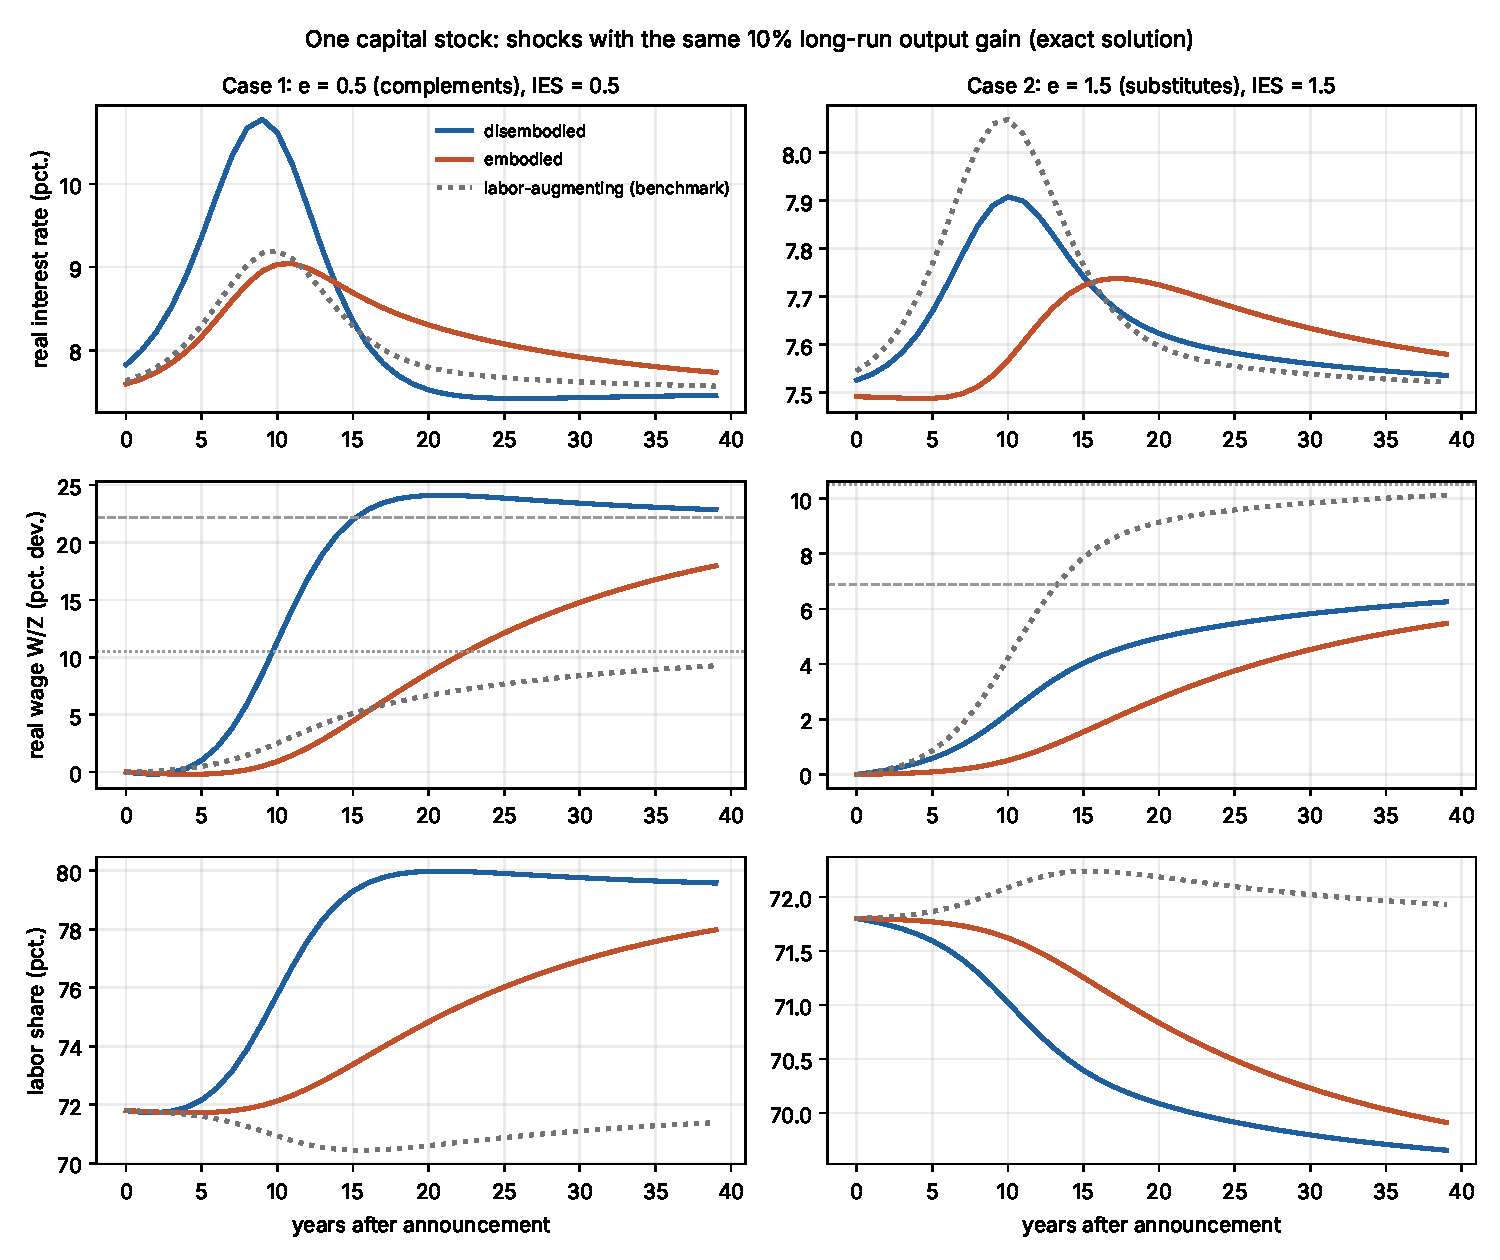
\includegraphics[width=\textwidth]{figures/fig_case12_exact.pdf}
\caption{Cases 1 and 2, exact solution ($\psi=\e$). Shocks have the same 10\% long-run output gain. Dashed lines: long-run wage $\gamma_Y/\e$; dotted: $\gamma_Y$.}\label{fig:c12}
\end{figure}

\begin{table}[t]\centering\scriptsize
\caption{Cases 1 and 2, exact solution ($\psi=\e$). Peak $r$ and the wage at $t{=}10$ are for the S-curve; $r_1$ (between years 0 and 1) is for a surprise step. The last column is the cumulative deviation of $\ln(1+r)$ from 7.5\% over 150 years.}\label{tab:c12}
\textbf{Case 1, $\e=0.5$}\\[2pt]\begin{tabular}{lcccccccc}\toprule
 & shock & peak $r$ & year & $r_1$, step & $W$, $t{=}10$ & $W$, long run & labor share & $\sum\Delta\ln(1+r)$\\
 & (log) & (pct.) & & (pct.) & (pct.) & (pct.) & long run (pct.) & (pct.)\\\midrule
Disembodied & 0.623 & 10.77 & 9 & 6.94 & 11.4 & 22.1 & 79.4 & 26.5\\
Embodied & 0.623 & 9.04 & 11 & 8.81 & 0.9 & 22.1 & 79.4 & 29.5\\
Labor-augmenting & 0.100 & 9.19 & 10 & 7.86 & 2.5 & 10.5 & 71.8 & 20.0\\
\bottomrule\end{tabular}
\\[6pt]
\textbf{Case 2, $\e=1.5$}\\[2pt]\begin{tabular}{lcccccccc}\toprule
 & shock & peak $r$ & year & $r_1$, step & $W$, $t{=}10$ & $W$, long run & labor share & $\sum\Delta\ln(1+r)$\\
 & (log) & (pct.) & & (pct.) & (pct.) & (pct.) & long run (pct.) & (pct.)\\\midrule
Disembodied & 0.160 & 7.91 & 10 & 7.72 & 2.2 & 6.9 & 69.4 & 6.0\\
Embodied & 0.160 & 7.74 & 17 & 7.90 & 0.5 & 6.9 & 69.4 & 5.6\\
Labor-augmenting & 0.100 & 8.07 & 10 & 7.61 & 4.2 & 10.5 & 71.8 & 6.7\\
\bottomrule\end{tabular}

\end{table}

\paragraph{Dynamics (Figure~\ref{fig:c12}, Table~\ref{tab:c12}).}
\begin{enumerate}
\item \emph{Interest rates, S-curve.} Disembodied progress raises $r$ sooner and
higher than embodied progress in both cases (case 1: 10.8 vs 9.0 percent at the peak;
case 2: 7.9 vs 7.7 percent). The embodied response peaks later (year 11 vs 9 in case 1,
year 17 vs 10 in case 2) and lasts longer. In case 2 the interest-rate response to
capital-specific progress is \emph{smaller} than to labor-augmenting progress of equal
long-run size (peak 8.1 percent). In case 1, disembodied progress raises $r$ more than
labor-augmenting progress (peak 9.2 percent). Complementary capital needs a much larger
technology shock (0.62 vs 0.16 log points) to deliver the same output gain, and its
effect is concentrated in the transition.
\item \emph{Interest rates, surprise step.} The ranking reverses on impact.
Embodied progress raises $r_1$ more (case 1: 8.8 vs 6.9 percent; case 2: 7.9 vs 7.7
percent). With complements, a disembodied step \emph{lowers} $r$ below its initial level.
Less investment is needed to reach the new capital stock, so the saving rate falls
(from 0.162 to 0.119), consumption jumps and then grows slowly.
\item \emph{Wages.} Embodied progress delays wage gains by about a decade: at year 10
wages are up 0.9 vs 11.4 percent in case 1 and 0.5 vs 2.2 percent in case 2.
Disembodied progress with complements pushes the wage temporarily above its long-run gain.
\item \emph{Labor share.} It moves in opposite directions in the two cases, and it moves
faster under disembodied progress. Labor-augmenting progress leaves it unchanged in the
long run.
\end{enumerate}
Proposition~\ref{prop:exact} requires $\psi=\e$, which ties complements to a low
intertemporal elasticity and substitutes to a high one. With log utility in both cases
(solved numerically, Appendix Table~\ref{tab:c12log}), the orderings are unchanged and
the magnitudes are similar. In case 1 the interest-rate effects are smaller because the
IES is higher.

\section{Case 3: regular capital and AI capital (numerical)}

Production nests a traditional bundle inside a CES with AI:
\begin{equation*}
X=\big[b_K(\Gamma_KK)^{\rho_1}+b_L(ZN)^{\rho_1}\big]^{1/\rho_1},\qquad
Y=\big[c_XX^{\rho_2}+c_A(\Gamma_AA)^{\rho_2}\big]^{1/\rho_2},
\end{equation*}
with $\e_1\le1$ (regular capital is a complement to labor; Cobb-Douglas in the
baseline, $\e_1=0.5$ as an alternative) and $\e_2=1.5$ (AI substitutes for both labor and
regular capital). AI starts small, with a 3 percent income share. Each stock accumulates through
(\ref{eq:acc}) with its own nest's elasticity. Utility is logarithmic.

\paragraph{No closed form.} The exact solutions require output and continuation value
to be linear in each $K_j^{\rho}$ for a single $\rho$. Here $X^{\rho_2}$ is not linear in
$K^{\rho_1}$ unless $\e_1=\e_2$, which would make AI and regular capital the same kind of input.
The one exception is $\e_1=\e_2=1$ with log utility, where everything is Cobb-Douglas and
AI is neither a substitute nor a complement. Case 3 is therefore solved as a
perfect-foresight Newton problem. The residuals are below $10^{-11}$ in every
experiment (Appendix).

\paragraph{A useful equivalence.} With a Cobb-Douglas bundle, capital-augmenting
progress in $K$ is the same as labor-augmenting progress: $\Gamma_K^{\sigma}(ZN)^{1-\sigma}$
with $\sigma$ the bundle's capital share. The two give identical paths for every
variable, which the numerical results reproduce exactly. In this baseline, the
relevant comparison is \emph{AI progress versus all conventional progress}.

\begin{figure}[p]\centering
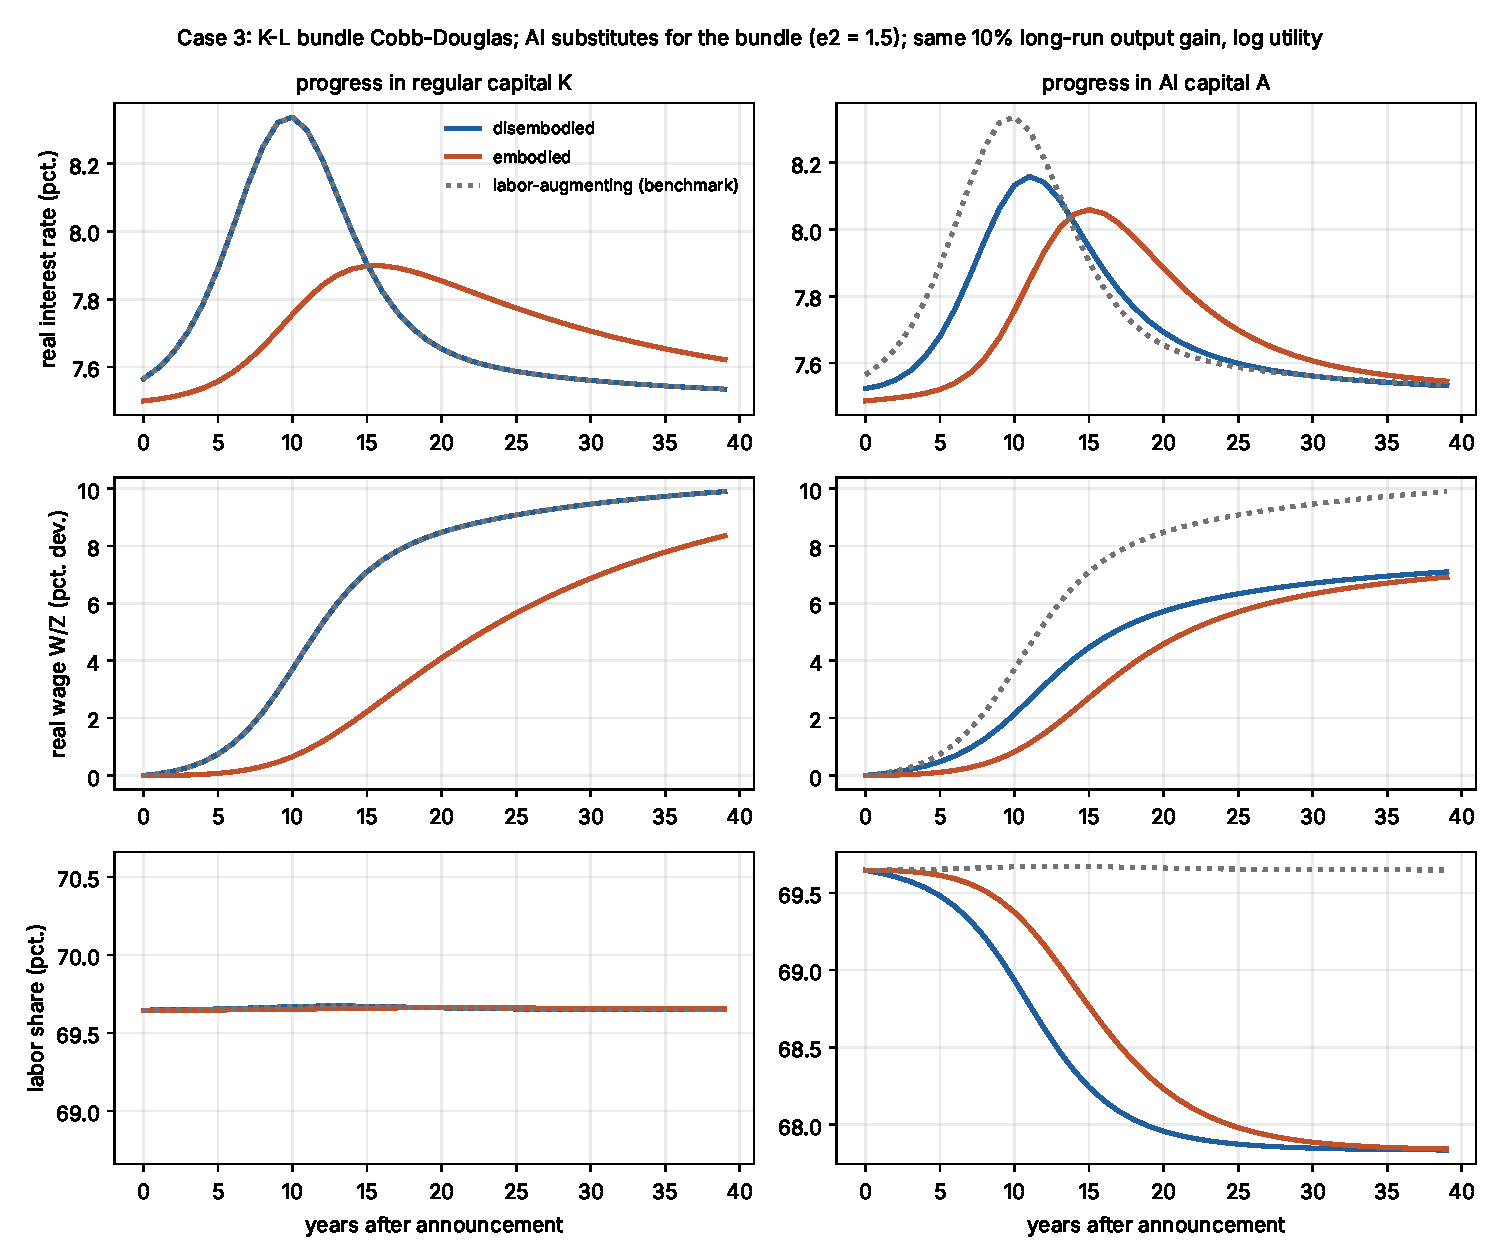
\includegraphics[width=\textwidth]{figures/fig_case3.pdf}
\caption{Case 3 (Cobb-Douglas bundle, $\e_2=1.5$, log utility): progress in regular capital versus AI capital, same 10\% long-run output gain.}\label{fig:c3}
\end{figure}

\begin{table}[t]\centering\scriptsize
\caption{Case 3. Top: Cobb-Douglas bundle (baseline). Bottom: CES bundle with $\e_1=0.5$. Columns as in Table~\ref{tab:c12}.}\label{tab:c3}
\textbf{Cobb-Douglas bundle}\\[2pt]\begin{tabular}{lcccccccc}\toprule
 & shock & peak $r$ & year & $r_1$, step & $W$, $t{=}10$ & $W$, long run & labor share & $\sum\Delta\ln(1+r)$\\
 & (log) & (pct.) & & (pct.) & (pct.) & (pct.) & long run (pct.) & (pct.)\\\midrule
$K$ disembodied & 0.255 & 8.34 & 10 & 7.71 & 3.7 & 10.5 & 69.6 & 10.0\\
$K$ embodied & 0.255 & 7.90 & 16 & 8.09 & 0.7 & 10.5 & 69.6 & 10.0\\
AI disembodied & 1.223 & 8.16 & 11 & 8.29 & 2.1 & 7.6 & 67.8 & 8.3\\
AI embodied & 1.223 & 8.06 & 15 & 9.18 & 0.8 & 7.6 & 67.8 & 8.1\\
Labor-augmenting & 0.100 & 8.34 & 10 & 7.71 & 3.7 & 10.5 & 69.6 & 10.0\\
\bottomrule\end{tabular}
\\[6pt]
\textbf{CES bundle, $\e_1=0.5$}\\[2pt]\begin{tabular}{lcccccccc}\toprule
 & shock & peak $r$ & year & $r_1$, step & $W$, $t{=}10$ & $W$, long run & labor share & $\sum\Delta\ln(1+r)$\\
 & (log) & (pct.) & & (pct.) & (pct.) & (pct.) & long run (pct.) & (pct.)\\\midrule
$K$ disembodied & 0.623 & 9.17 & 9 & 7.31 & 12.2 & 22.1 & 77.0 & 13.5\\
$K$ embodied & 0.623 & 8.30 & 11 & 8.17 & 1.5 & 22.1 & 77.0 & 14.9\\
AI disembodied & 1.327 & 8.27 & 11 & 8.42 & 2.3 & 8.5 & 68.4 & 8.6\\
AI embodied & 1.327 & 8.15 & 15 & 9.54 & 0.9 & 8.5 & 68.4 & 8.4\\
Labor-augmenting & 0.100 & 8.39 & 10 & 7.73 & 3.1 & 10.5 & 69.6 & 10.2\\
\bottomrule\end{tabular}

\end{table}

\paragraph{Results (Figure~\ref{fig:c3}, Table~\ref{tab:c3}).}
\begin{enumerate}
\item \emph{Long-run wages.} With the same 10 percent output gain, AI progress raises
the wage by 7.6 percent against 10.5 percent for conventional progress, and the labor
share falls from 69.6 to 67.8 percent. With a complementary bundle ($\e_1=0.5$), the
contrast is starker. Regular-capital progress raises wages by 22 percent, as in case 1,
while AI progress raises them by 8.5 percent.
\item \emph{Size of the technology shock.} Because AI starts small, the same output gain
needs a large improvement in AI technology: $\Gamma_A/P_A$ rises 3.4-fold
($e^{1.22}$), against a 29 percent rise for regular capital. The AI share of income
grows along the way.
\item \emph{Interest rates.} For a gradual S-curve, peak effects are similar. Disembodied
AI progress peaks slightly below conventional progress (8.2 vs 8.3 percent), and embodied
AI progress slightly above embodied regular-capital progress (8.1 vs 7.9 percent). For a surprise step, AI progress raises $r$ \emph{more} on impact:
8.3 vs 7.7 percent if disembodied, and 9.2 vs 8.1 percent if embodied. The AI investment
boom is large relative to its initial stock, so the long-run saving rate rises from 0.181
to 0.196, and in the meantime consumption grows faster.
\item \emph{Embodied versus disembodied.} The pattern of cases 1 and 2 carries over.
Embodied progress gives a later, more persistent rise in $r$, a slower rise in wages
(0.8 vs 2.1 percent at year 10 for AI) and a larger impact effect after a surprise step.
\end{enumerate}

\section{Summary}

\begin{itemize}
\item \emph{Long run} (closed form in cases 1 and 2). For the same output gain, the wage
rises by $\gamma_Y/\e$ under capital-specific progress, against $\gamma_Y$ under
labor-augmenting progress. If AI substitutes for labor, workers gain less than output and
the labor share falls. The long-run interest rate is unchanged by level shifts in
technology, and embodied and disembodied progress have identical long-run effects.
\item \emph{Dynamics.} Disembodied AI progress (better models applied to installed
compute and software) raises interest rates early and lifts wages quickly. Embodied AI
progress (cheaper new AI capital) works through an investment boom. Its rise in rates
is delayed and more persistent, and its wage gains lag by a decade. A surprise step
raises rates more under embodied progress.
\item \emph{AI versus conventional progress} (case 3, numerical). AI progress yields
smaller wage gains, a falling labor share, a higher saving rate and a larger
impact effect on the real rate after news. Its peak interest-rate effect under gradual
diffusion is similar to that of conventional progress.
\end{itemize}

\appendix
\section{Robustness and verification}

\begin{table}[h]\centering\scriptsize
\caption{Cases 1 and 2 with log utility ($\psi=1$), solved numerically.}\label{tab:c12log}
\textbf{Case 1, $\e=0.5$}\\[2pt]\begin{tabular}{lcccccccc}\toprule
 & shock & peak $r$ & year & $r_1$, step & $W$, $t{=}10$ & $W$, long run & labor share & $\sum\Delta\ln(1+r)$\\
 & (log) & (pct.) & & (pct.) & (pct.) & (pct.) & long run (pct.) & (pct.)\\\midrule
Disembodied & 0.623 & 9.21 & 9 & 7.20 & 12.3 & 22.1 & 79.4 & 13.6\\
Embodied & 0.623 & 8.32 & 10 & 8.20 & 1.5 & 22.1 & 79.4 & 15.0\\
Labor-augmenting & 0.100 & 8.41 & 10 & 7.69 & 3.1 & 10.5 & 71.8 & 10.3\\
\bottomrule\end{tabular}
\\[6pt]
\textbf{Case 2, $\e=1.5$}\\[2pt]\begin{tabular}{lcccccccc}\toprule
 & shock & peak $r$ & year & $r_1$, step & $W$, $t{=}10$ & $W$, long run & labor share & $\sum\Delta\ln(1+r)$\\
 & (log) & (pct.) & & (pct.) & (pct.) & (pct.) & long run (pct.) & (pct.)\\\midrule
Disembodied & 0.160 & 8.07 & 10 & 7.80 & 2.1 & 6.9 & 69.4 & 8.8\\
Embodied & 0.160 & 7.84 & 17 & 8.05 & 0.4 & 6.9 & 69.4 & 8.4\\
Labor-augmenting & 0.100 & 8.30 & 10 & 7.66 & 4.0 & 10.5 & 71.8 & 9.8\\
\bottomrule\end{tabular}

\end{table}

\begin{figure}[h]\centering
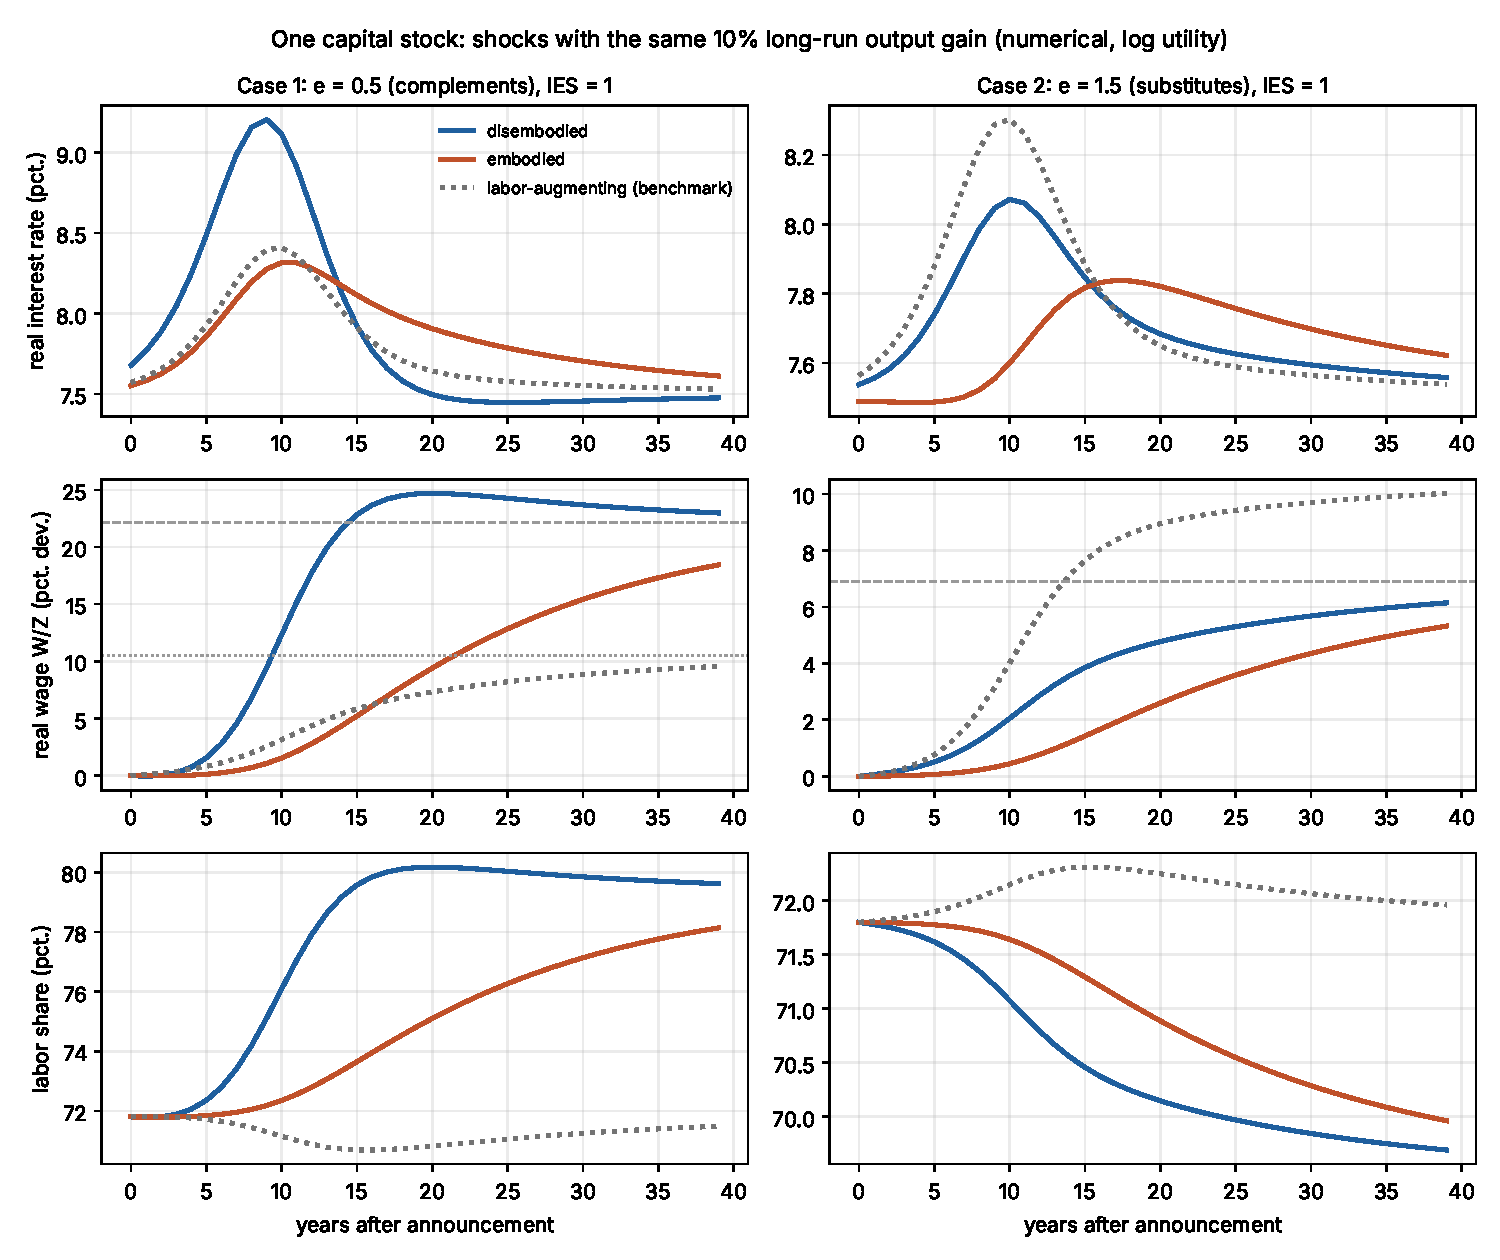
\includegraphics[width=\textwidth]{figures/fig_case12_log.pdf}
\caption{Cases 1 and 2 with log utility ($\psi=1$).}
\end{figure}

\begin{figure}[h]\centering
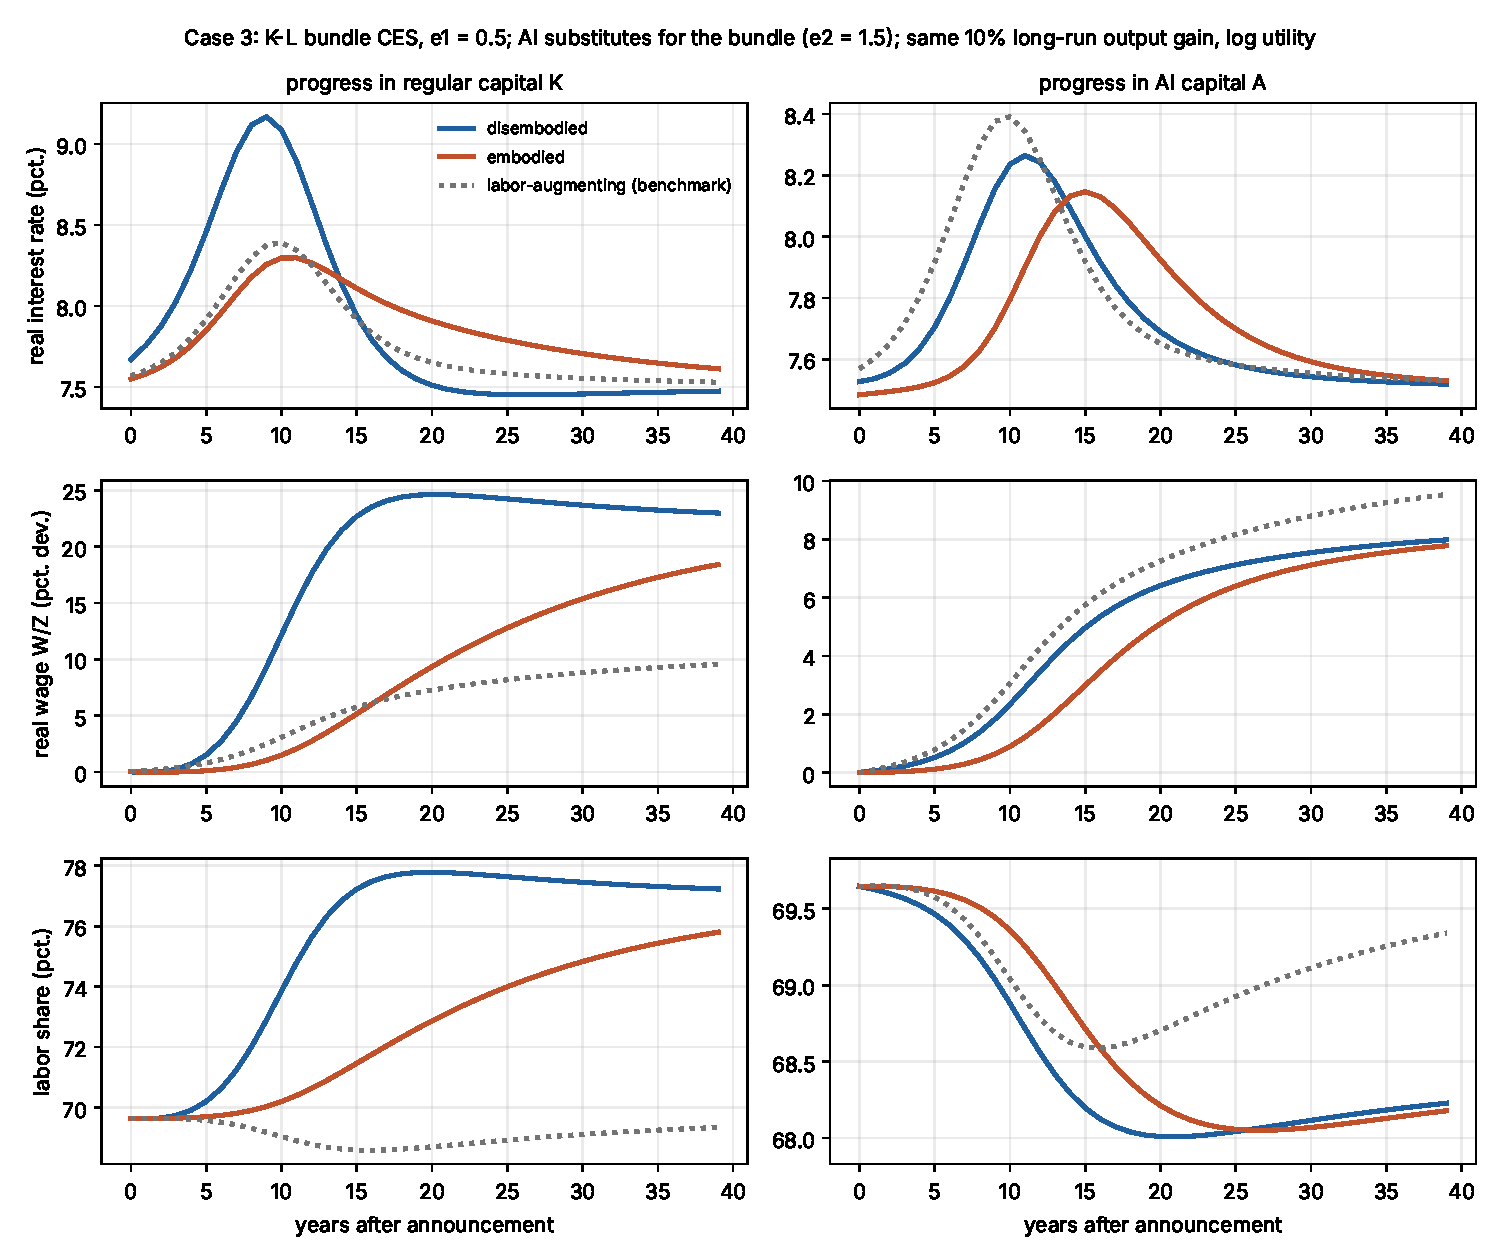
\includegraphics[width=\textwidth]{figures/fig_case3_ces.pdf}
\caption{Case 3 with a CES bundle ($\e_1=0.5$).}
\end{figure}

\texttt{cases.py} computes everything. For cases 1 and 2 it compares the
backward-recursion saving rates of Proposition~\ref{prop:exact} with a generic Newton
solve of the Euler equations started 5 percent away. It checks the shock sizes and long-run
wage formulas of Proposition~\ref{prop:lr}, and it reports Newton residuals for case 3.

\begin{table}[h]\centering\scriptsize
\caption{Verification.}
\begin{tabular}{lc}\toprule Check & max abs. error\\\midrule
case1: shock size = closed form (dis) & 6.7e-16\\
case1 dis S: generic = exact s & 8.6e-16\\
case1 dis step: generic = exact s & 8.7e-16\\
case1: shock size = closed form (emb) & 4.4e-16\\
case1 emb S: generic = exact s & 8.7e-16\\
case1 emb step: generic = exact s & 8.7e-16\\
case1 Z S: generic = exact s & 1.1e-15\\
case1 Z step: generic = exact s & 1.1e-15\\
case1 IES=exact: long-run ln W = target/e (dis) & 1.7e-16\\
case1 IES=exact: long-run ln W = target/e (emb) & 1.9e-16\\
case1 IES=exact: long-run ln W = target (Z) & 6.9e-17\\
case1 IES=log: long-run ln W = target/e (dis) & 1.7e-16\\
case1 IES=log: long-run ln W = target/e (emb) & 1.9e-16\\
case1 IES=log: long-run ln W = target (Z) & 6.9e-17\\
case2: shock size = closed form (dis) & 6.7e-16\\
case2 dis S: generic = exact s & 1.2e-12\\
case2 dis step: generic = exact s & 1.2e-12\\
case2: shock size = closed form (emb) & 4.9e-14\\
case2 emb S: generic = exact s & 1.1e-12\\
case2 emb step: generic = exact s & 1.3e-12\\
case2 Z S: generic = exact s & 1.1e-12\\
case2 Z step: generic = exact s & 1.1e-12\\
case2 IES=exact: long-run ln W = target/e (dis) & 1.4e-16\\
case2 IES=exact: long-run ln W = target/e (emb) & 1.2e-15\\
case2 IES=exact: long-run ln W = target (Z) & 6.9e-17\\
case2 IES=log: long-run ln W = target/e (dis) & 1.4e-16\\
case2 IES=log: long-run ln W = target/e (emb) & 1.2e-15\\
case2 IES=log: long-run ln W = target (Z) & 6.9e-17\\
case3: initial steady state reproduces calibration & 1.4e-17\\
case3 disK S: Newton residual & 1.9e-14\\
case3 disK step: Newton residual & 5.9e-12\\
case3 embK S: Newton residual & 1.8e-15\\
case3 embK step: Newton residual & 5.0e-15\\
case3 disA S: Newton residual & 4.8e-13\\
case3 disA step: Newton residual & 2.9e-15\\
case3 embA S: Newton residual & 6.9e-13\\
case3 embA step: Newton residual & 5.9e-14\\
case3 Z S: Newton residual & 1.9e-14\\
case3 Z step: Newton residual & 5.9e-12\\
case3 ces: initial steady state reproduces calibration & 1.4e-17\\
case3 ces disK S: Newton residual & 6.5e-12\\
case3 ces disK step: Newton residual & 2.8e-15\\
case3 ces embK S: Newton residual & 3.4e-15\\
case3 ces embK step: Newton residual & 2.6e-13\\
case3 ces disA S: Newton residual & 6.5e-13\\
case3 ces disA step: Newton residual & 3.0e-13\\
case3 ces embA S: Newton residual & 8.1e-13\\
case3 ces embA step: Newton residual & 5.8e-12\\
case3 ces Z S: Newton residual & 4.2e-13\\
case3 ces Z step: Newton residual & 2.1e-15\\
\bottomrule\end{tabular}

\end{table}

\begin{thebibliography}{9}
\bibitem[Kiley(2000)]{kiley2000}
Kiley, M.~T. (2000). ``Stock Prices and Fundamentals in a Production Economy.''
FEDS Working Paper 2000-05, Federal Reserve Board.
\bibitem[Kiley(2004)]{kiley2004}
Kiley, M.~T. (2004). ``Stock Prices and Fundamentals: A Macroeconomic Perspective.''
\emph{Journal of Business} 77(4): 909--936.
\end{thebibliography}
\end{document}
